\section{Conventional Methods in Action Recognition}
META: 
Condensed overview and description of conventional Methods in action Recognition using the taxonomy of Aggarwal and Ryoo's fine survey paper.
More detailed description of methods using local-features, since these have become the standard approach in action recognition after Aggarwal and Ryoo's overview.

\begin{figure}[H]
    \centering
    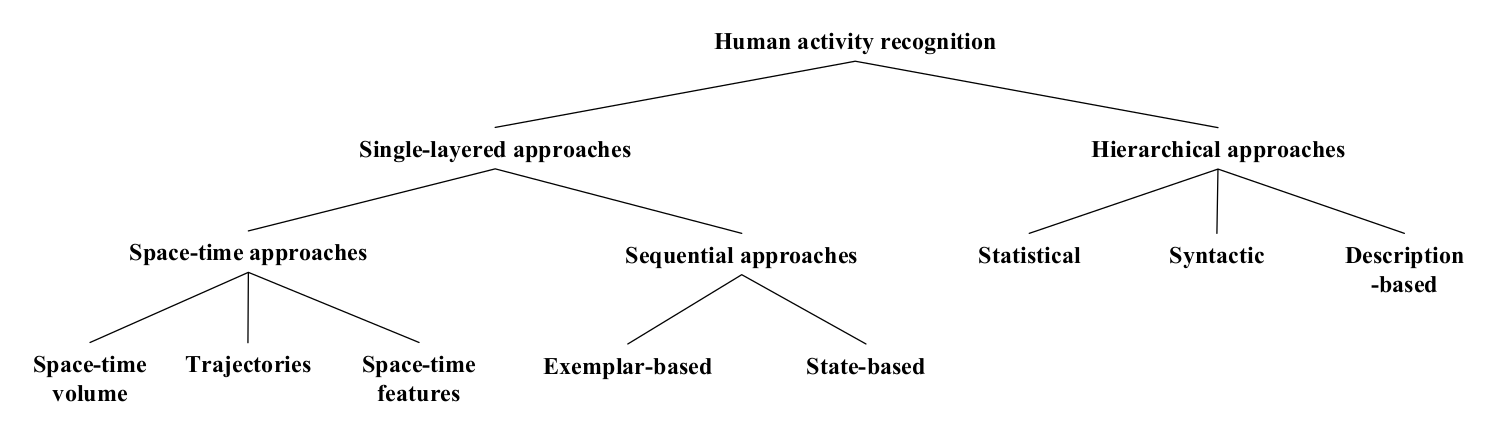
\includegraphics[width=\textwidth]{img_conventional/taxonomy_conventional_methods.png}
    \caption{Approach-based taxonomy for conventional methods in human activity recognition as given by Aggarwal and Ryoo\cite{aggarwal_human_2011}}
    \label{fig:conventional_taxonomy}
\end{figure}

3 Main components in action recognition using local features: Feature Extraction, Representation Building, Classification.

Methods for feature extraction: Interest point detectors or dense sampling.

Space-time interest point detectors: Harris3D\cite{laptev_space-time_2005}, Cuboids\cite{dollar_behavior_2005}, Hessian Detector\cite{willems_efficient_2008}

Descriptors for 3D volumes around previously detected space-time interest points: Histogram of Gradient HOG\cite{dalal_histograms_2005-1}, Histogram of Optical Flow (HOF)\cite{laptev_learning_2008}, 3D Histogram of Gradient (HOG3D)\cite{klaser_spatio-temporal_2008}, Extended SURF (ESURF)\cite{willems_efficient_2008}

``standard approach to video classification'' described in \cite{karpathy_large-scale_2014}

Laptev and Lindeberg [26] proposed spatio-temporal interest points (STIPs)
by extending Harris corner detectors to 3D. SIFT and HOG
are also extended into SIFT-3D [34] and HOG3D [19] for
action recognition. Dollar et al. proposed Cuboids features
for behavior recognition [5]. Sadanand and Corso built Ac-
tionBank for action recognition [33]. Recently, Wang et al.
proposed improved Dense Trajectories (iDT) [44] which is
currently the state-of-the-art hand-crafted feature. Tran 2015

other iDT-based methods: Beyond gaussian pyramid: Multi-skip feature stacking for action recognition.
Bag of visual words and fusion methods for action recognition: Comprehensive study and good practice.

Recently, interest point detectors and local descriptors have
been extended from images to videos. Laptev and Linde-
berg [13] introduced space-time interest points by extend-
ing the Harris detector. Other interest point detectors in-
clude detectors based on Gabor filters [1, 5] or on the de-
terminant of the spatio-temporal Hessian matrix [33]. Fea-
ture descriptors range from higher order derivatives (local
jets), gradient information, optical flow, and brightness in-
formation [5, 14, 24] to spatio-temporal extensions of image descriptors, such as 3D-SIFT [25], HOG3D [11], extended
SURF [33], or Local Trinary Patterns [34]. Action Recognition by dense trajectories -- Wang 2011

\subsection{Overview}

\subsection{Local Features}

Interest point detection: Space-time interest points ``I. Laptev. On space-time interest points. IJCV, 64(2-3), 2005.''

Local feature approaches extract features, i.e\ different characteristics of pixel values of a video, in locally limited neigbourhoods.
The algorithm to extract these features is called a feature extractor.

Three main questions:
\begin{enumerate}
    \item Where to the features (around what points?)
    \item What features to extract?
    \item How to aggregate the extracted feature (vectors) into a global fixed-size representation of the video.
\end{enumerate}

\subsubsection{Feature extractors}

Cuboids ``P. Dollár, V. Rabaud, G. Cottrell, and S. Belongie. Behavior recognition via sparse spatio-temporal features. In VS-PETS, 2005.''

\subsubsection{Aggregation Methods}

\textbf{Bag of visual Words paradigm}

Can be improved with a multi-channel approach as in ``M. M. Ullah, S. N. Parizi, and I. Laptev. Improving bag-of-features action recognition with non-local cues. In BMVC,2010.''

\textbf{Fisher Vector}

One limitation of these local features is that they lack semantics and discriminative capacity. Therefore mid-level and high-level features were proposed (cite TDD).

\subsection{State of the Art Approaches using locaf features}

\subsubsection{Action Recognition by Dense Trajectories -- Wang et al. (2011)}

\textcite{wang_action_2011} introduce a tracking technique called \textit{dense trajectories} for action classification from videos.

Points are sampled densely from each frame and then tracked using a dense optical flow field.

Local features are extracted along the resulting point trajectories to form trajectory descriptors, which are then aggregated into a global video descriptor using the bag-of-words paradigm. cite ??

Before, also other approaches used feature trajectories for action recognition by either tracking sparse spatio-temporal interest points using a standard KLT tracker or by matching SIFT features between consecutive frames.

Dense sampling of interest points has shown to yield improved performance in action recognition over sparse spatio-temporal interest points \cite{wang_evaluation_2009}.
However using the KLT tracker to obtain dense trajectories or matching SIFT features on densely sampled points would be computationally too expensive to handle large datasets. 
The authors approach therefore represents an efficient way to extract dense trajectories.

Since motion in a video, and therefore trajectories can stem from either motion of interest or unwanted camera motion, the authors propose using a descriptor called \textit{Motion Boundary Histogram} (MBH), which aims at focussing on foreground motion.
The motion boundary histogram descriptor is designed to make the classification of actions in a video invariant to camera motion.

The overall approach for obtaining a descriptor along densely extracted trajectories is shown in figure \ref{fig:densetrajectories_approach}

\begin{figure}[H]
    \centering
    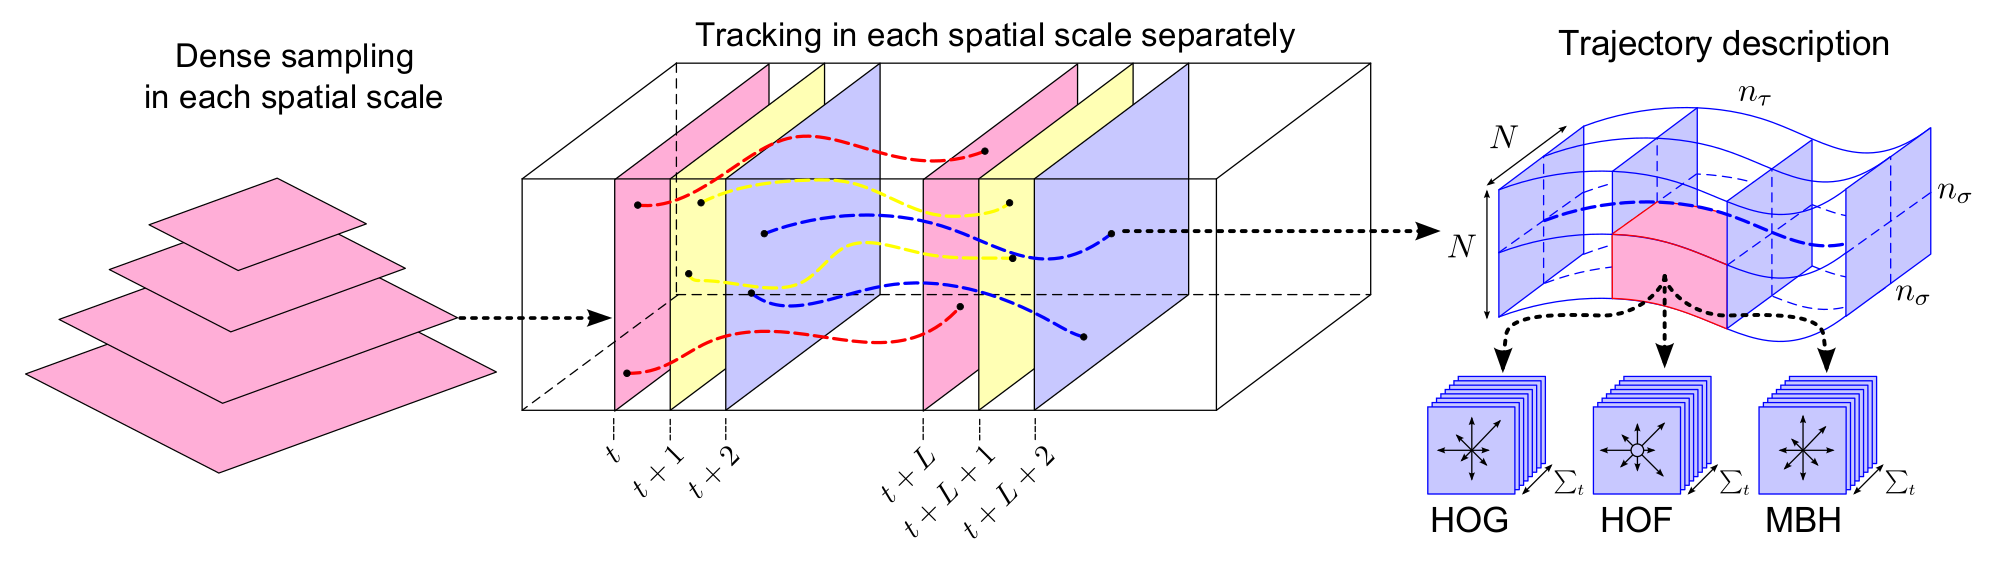
\includegraphics[width=\textwidth]{img_conventional/densetrajectories_approach}
    \caption{Description of densely extracted trajectories \cite{wang_action_2011}}
    \label{fig:densetrajectories_approach}
\end{figure}

Dense trajectories are obtained separately from 8 spatial scales, which differ by a factor of $1 / \sqrt{2}$.
Points are sampled on a grid spaced by $W$ pixels on each scale. Experimentally $W = 5$ has been shown to yield good results.

Each point $P_t$ at frame $t$ is tracked to the next frame by mean-filtering a dense optical flow field, which was extracted by the Farnebäck algorithm \cite{farneback_two-frame_2003} as implemented in OpenCV.
The tracked points in subsequent frames then form the trajectory $(P_t, P_{t+1}, P_{t+2}, \cdots)$.

The maximum length of a trajectory is limited to $L = 15$ frames to avoid the problem of drifting.
Trajectories that exceed this limit are removed from the tracking process.
The presence of a trackectory in each $W \times W$ unit of each frame is verified. If no tajectory is present, a new point is sampled and added to the tracking process.

Since only dynamic information is important for action recognition, static trajectories are removed in a pre-processing stage.
Erroneous trajectories with sudden large displacements are also removed.

A simple descriptor is obtained from the shape information given by the trajectory.
It is formed by normalizing the spatial displacements given by the differences of consecutive points in a trajectory.
Formally the \textit{trajectory descriptor} $S'$ is given by:
\begin{equation*}
    S' = \frac{(\Delta P_t, \cdots, \Delta P_{t+L-1})}{\sum_{j=t}^{t+L-1} \|P_j\|}
\end{equation*}
Where $\Delta P_t = (P_{t+1} - P_t) = (x_{t+1} - x_t, y_{t+1} - y_t)$.

\textbf{Local Feature Descriptors:}\\
Local features are extracted from video volumes of size $N \times N \times L$ around the trajectories as depicted in figure \ref{fig:densetrajectories_approach}, where $N = 32$ has shown to yield good results.

Feature descriptors evaluated in the context of dense trajectories are (see also ??):
\begin{itemize}
    \item \textbf{HOG} (Histogram of Oriented Gradients) \cite{dalal_histograms_2005-1}
    \item \textbf{HOF} (Histogram of Optical Flow) \cite{laptev_learning_2008}
    \item \textbf{MBH} (Motion Boundary Histogram) \cite{dalal_human_2006}
\end{itemize}

\begin{figure}[H]
    \centering
    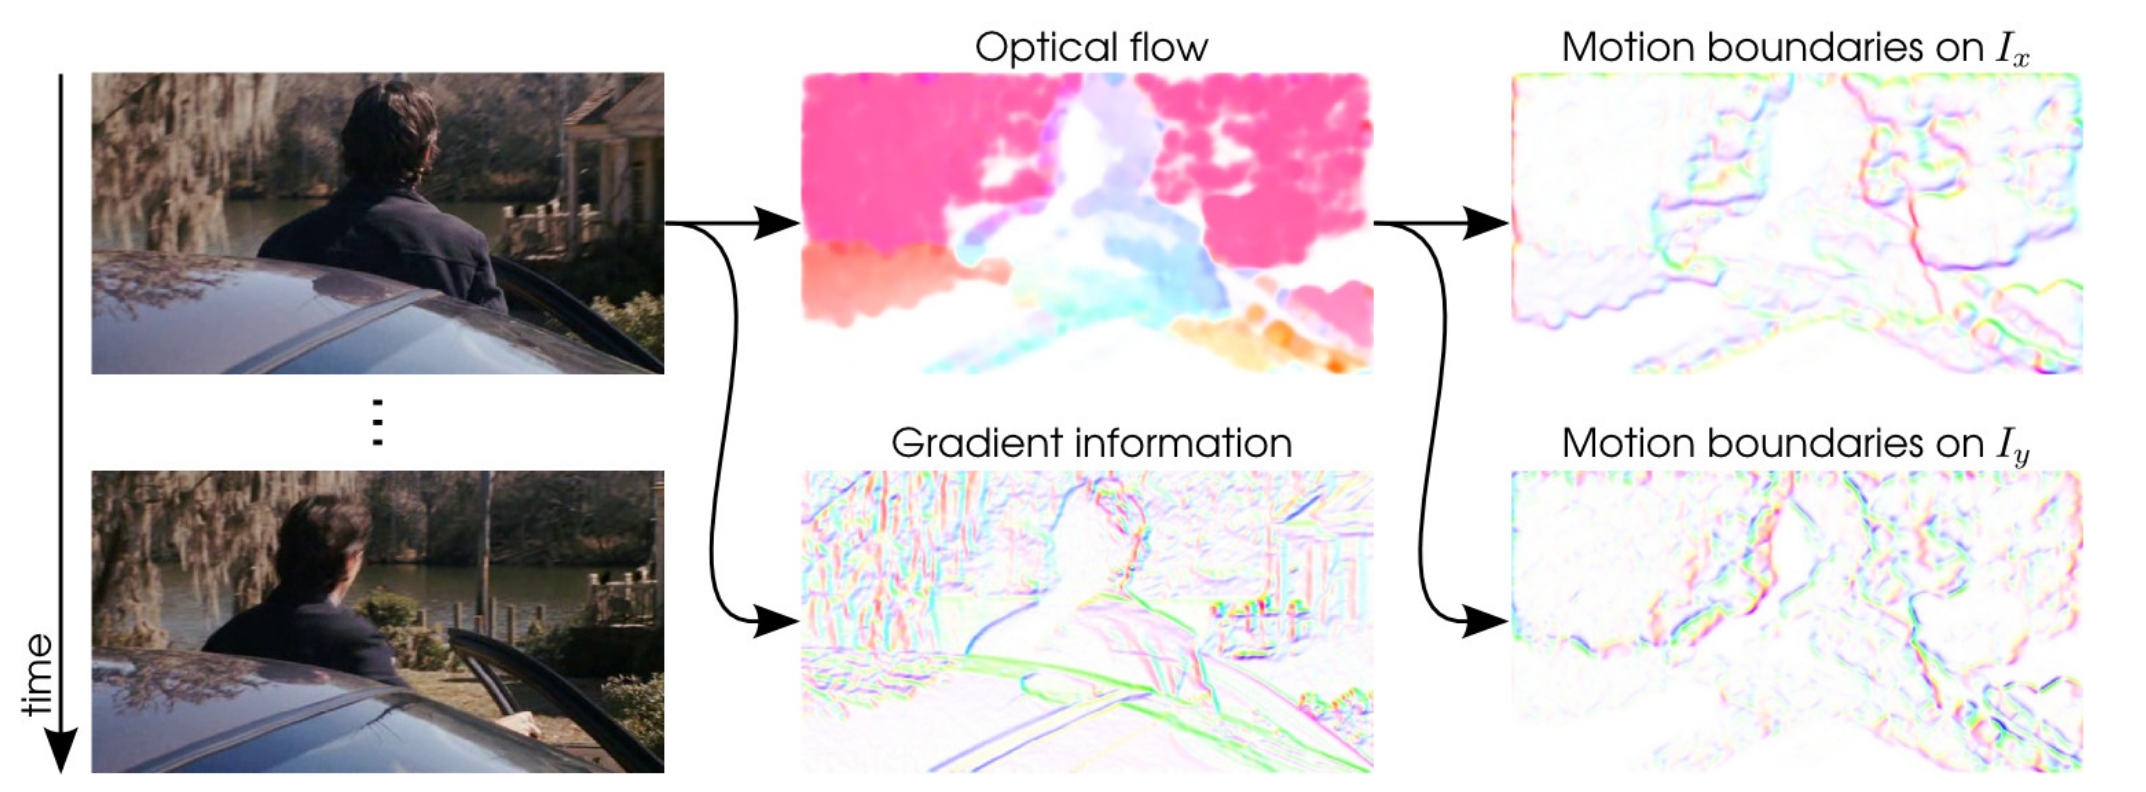
\includegraphics[width=\textwidth]{img_conventional/densetrajectories_featurevisualization}
    \caption{Visualization of the information captured by HOG, HOF and MBH on complete video frames. In each image, the orientation is given by color, the magnitude is given by saturation. \cite{wang_action_2011}}
    \label{fig:densetrajectories_featurevisualization}
\end{figure}

The HOG descriptor encodes static appearance information by computing the orientations of image gradients and aggregating them in a histogram over all subframes of the current video volume along the trajectory. In this approach the histograms contain 8 bins.

The HOF descriptor aggregates the orientations of optical flow vectors in a histogram and therefore captures local motion information. An additional bin is used here, i.e.\ 9 bins.

The MBH descriptor separately calculates the spatial derivatives of the $x$- and $y$-component of the optical flow field.
The orientations of the derivatives are aggregated into histograms (similarly to the HOG descriptor), which represent the video volume.
An advantage of MBH is that is suppresses constant motion, since it takes only the changes in the flow field (i.e.\ motion boundaries) into account.
The authors therefore use MBH as an easy way to filter noise stemming from background camera-motion (compare the optical flow-image and motion boundaries in figure \ref{fig:densetrajectories_featurevisualization}).

The authors evaluate their approach on the KTH, YouTube, Hollywood2 and UCF-Sports dataset using a standard bag-of-features approach as follows:

\begin{enumerate}
    \item Construction of a codebook for each descriptor-type (trajectory, HOG, HOF and MBH).
        $100.000$ descriptors for each type are randomly chosen from all extracted descriptors over the dataset's training split.
        These descriptors are clustered into a 4000 words long codebook using $k$-means.
    \item Each extracted descriptor from a video is assigned to its nearest codebook-descriptor using the Euclidean distance.
        The number of occurences are aggregated in a histogram, which builds the global video descriptor.
    \item A classifier (here a non-linear SVM with a $\chi^2$ kernel) is trained to assign the class-labels to the global video descriptors.
\end{enumerate}

Different descriptor can be combined ??.

Besides densely sampled trajectories, the authors evaluate baseline trajectories obtained from the KLT tracker for comparison.
The same descriptors (trajectory, HOG, HOF and MBH) are used aorund the KLT-trajectories.

\begin{table}[H]
    \centering
    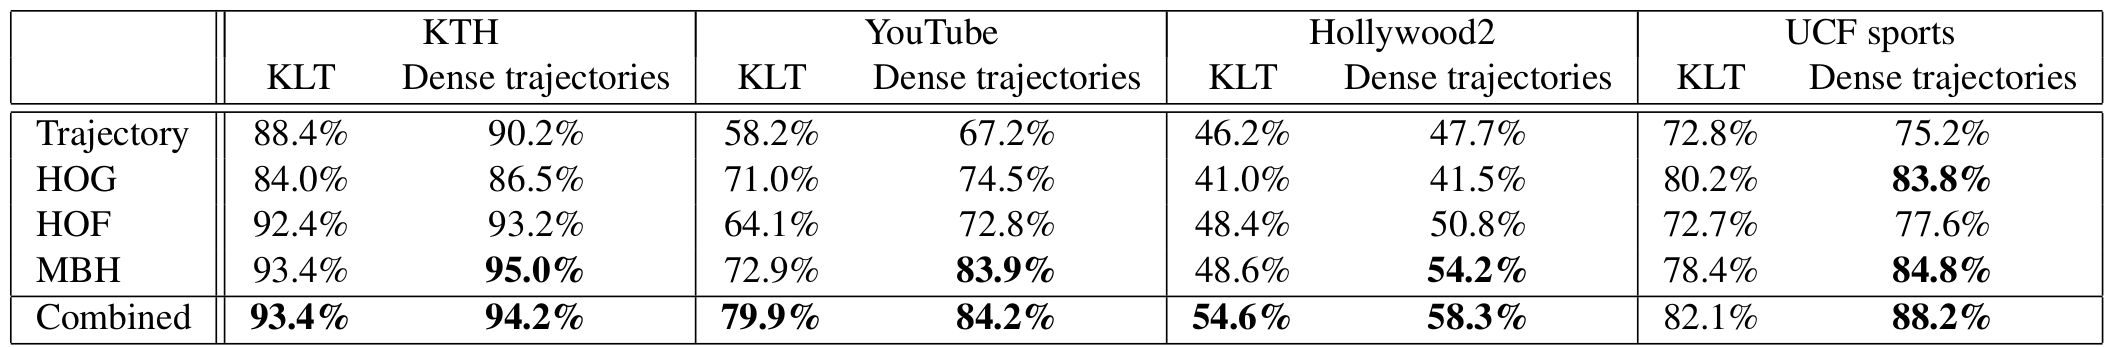
\includegraphics[width=\textwidth]{img_conventional/densetrajectories_results}
    \caption{Results of dense trajectories compared to KLT-trajectories when using different feature descriptors. \cite{wang_action_2011}}
    \label{tab:densetrajectories_results}
\end{table}

The results in table \ref{tab:densetrajectories_results} show the superiority of dense trajectories compared to the KLT baseline.

The simple trajectory descriptor yields surprisingly good results, which confirms the importance of motion information encoded in the trajectory shapes according to the authors.

The MBH descriptor performs significantly better than all the other descriptors.
On the youtube dataset, the advantage of using the MBH descriptor is most prominent, since the videos in this dataset contain a lot of noise from camera-motion (uncontrolled, realistic videos, often recorded by handheld cameras).

The dense trajectory approach significantly outperformed the state-of-the art on the YouTube, Hollywood2 and UCF Sports datasets when all descriptors are combined.
On the KTH dataset, the approach yields competitive results.

\subsubsection{Action recognition with improved trajectories -- Wang et al. (2013)}
\cite{wang_action_2013}

\subsubsection{Multi-view super vector for action recognition -- Cai et al. (2014)}
\cite{cai_multi-view_2014}

\subsubsection{Bag of visual words and fusion methods for action recognition: Comprehensive study and good practice -- Peng et al. (2014)}
\cite{peng_bag_2014}

